% Multiple Choice Question 31

\begin{center}
    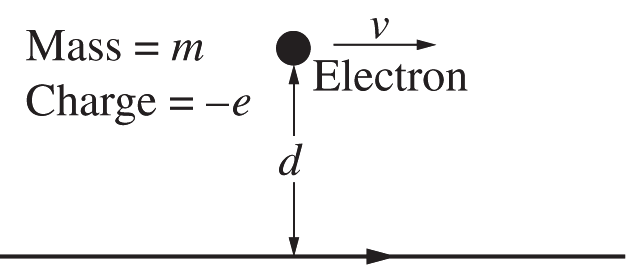
\includegraphics[scale=0.3]{images/img-014-027.png}
\end{center}

\begin{questions}
\setcounter{question}{30}

\question
An electron of mass $m$ and charge $-e$ is traveling to the right parallel to a wire with speed $v$. The electron is a distance $d$ from the wire. The wire is carrying a current $I$ to the right, as shown in the figure above. Which of the following gives the magnitude and direction of the force exerted on the electron by the current-carrying wire?

\tabto{0.75cm} \underline{Magnitude}
\tabto{4.00cm} \underline{Direction}

\begin{choices}
    \choice $\dfrac{\mu_{0} I e v}{2 \pi d}$   \tabto{3.25cm} Toward the top of the page
    \choice $\dfrac{\mu_{0} I e v}{2 \pi d}$   \tabto{3.25cm} Out of the page
    \choice $\dfrac{\mu_{0} I e v}{2 \pi d}$   \tabto{3.25cm} Into the page
    \choice $\dfrac{\mu_{0} I e v}{2 m \pi d}$ \tabto{3.25cm} Toward the top of the page 
    \choice $\dfrac{\mu_{0} I e v}{2 m \pi d}$ \tabto{3.25cm} Out of the page
\end{choices}

\end{questions}
